\documentclass{article}
\usepackage[spanish]{babel}
\usepackage{graphicx}

\author{Hernández Hernández Ángel, Juárez Botello Josué Adalid, Plata Salinas Eidan Owen, Trejo Arraiga Rodrigo Gerardo}
\title{Planeación ADS}

\begin{document}

\begin{titlepage}
	\centering
	
\includegraphics[height=2cm]{Logo_IPN.png}
	\hfill
	
\includegraphics[height=2cm]{escudoESCOM.png}

	\vspace{-1.5cm}
	\large\textbf{ Instituto Politécnico Nacional}\\
	\large\textbf{Escuela Superior de Cómputo}\\
	\large{Unidad Zacatenco}

	\vspace{2cm}

	\Large{\textbf{Análisis y Diseño de Sistemas}}

	\vspace{10cm}

	\begin{tabular}{rl}
		\textbf{Proyecto} & Planeación                    \\
		\textbf{Profesor} & Vélez Saldaña Ulises          \\
		\textbf{Equipo}
		                  & Hernández Hernández Ángel     \\
		                  & Juárez Botello Josué Adalid   \\
		                  & Plata Salinas Eidan Owen      \\
		                  & Trejo Arriaga Rodrigo Gerardo \\
	\end{tabular}
\end{titlepage}

\tableofcontents
\pagebreak

\section{Introducción}

Este documento tiene como objetivo presentar una propuesta para el desarrollo de un proyecto de software para la administración y gestión de información de niños en una guardería, así como la comunicación con sus tutores y el personal médico. En este análisis, se examinan los principales problemas que enfrenta la institución, así como las características del proyecto, incluyendo los riesgos asociados con la falta de conocimiento y experiencia en el desarrollo de proyectos similares.

A partir de este análisis, se proponen diversas soluciones que permitirían una gestión integral y personalizada de la información, mejorando la comunicación y coordinación entre los distintos actores involucrados en la guardería y optimizando la eficiencia en la gestión de la institución.

El documento también examina las tecnologías y herramientas que se utilizarán en el proyecto.

Este análisis también menciona brevemente los desafíos asociados con la falta de experiencia en proyectos largos y la mala organización del tiempo, así como las fortalezas del equipo, incluyendo conocimientos de programación estructurada, orientada a objetos, orientada a eventos, funcional y lógica, así como experiencia en desarrollo de aplicaciones web y sistemas distribuidos.

Los principales puntos a tratar son los problemas de la guardería y sus soluciones tratadas como requerimientos tentativos para el desarrollo de una aplicación web segu las necesidades del cliente y su negocio.

\section{Análisis del proyecto}
\subsection{Características del proyecto}


\begin{itemize}
	\item Entre los riesgos más destacables tenemos el que los requerimientos los vamos a ir descubriendo sobre la marcha, y que las cosas que son necesarias de nosotros pueden ir aumentando fuera de nuestro conocimiento.
	\item Se trata de una aplicación web responsable de la administración y gestión de información de niños en una guardería, así como de la comunicación con sus tutores y el personal médico de ser necesario.
	\item El programa a realizar tiene un tamaño mediano a comparación de otras guarderías debido a que no abarca un sistema completo de empleados ni atención médica, pero si contiene la administración de alumnos y docentes por aulas y grupos.
	\item Debido a que La arquitectura es: \emph{Modelo-Vista-Controlador} será más fácil trabajar con los datos sin sobrecargar a un único equipo de cómputo, al poder distribuir la base de datos en un dispositivo diferente al del controlador de ser necesario.
	\item No conocemos las tecnologías que vamos a utilizar en el proyecto, no sabemos completamente cuánto tiempo vamos a tener disponible para el desarrollo, sobrecarga de actividades, no tenemos buena organización y la metodología de trabajo la vamos a ir aprendiendo en paralelo al desarrollo del proyecto.

	\item Tenemos conocimientos de programación estructurada, orientada a objetos, orientada a eventos, funcional y algo de lógico, así como conocimientos básicos de bases de datos. Y algunos de los miembros del equipo cuentan con experiencia en desarrollo de aplicaciones web y sistemas distribuidos.

	\item Nuestra principal debilidad es la mala organización del tiempo y la falta de experiencia en desarrollo de proyectos largos.

	\item El proyecto es muy complejo de programar y diseñar varias partes del proyecto como la base de datos, especialmente las pantallas debido a que no tenemos a un diseñador gráfico. Pero se puede facilitar con el servicio \emph{REST}.

\end{itemize}

Con las siguientes tecnologías:
\begin{itemize}
	\item HTML 5, CSS, JavaScript.
	\item Spring Boot 3.0.5 (JDK LTS 17).
	\item PhpMyAdmin (\emph{MariaDB}).
\end{itemize}
\subsection{Metodología}
Incremental enfocado a Scrum.

\subsection{Ventajas y desventajas}

\subsubsection{Ventajas}
\begin{itemize}
	\item Flexibilidad: Es una metodología ágil que se adapta fácilmente a los cambios del proyecto y a los requerimientos del cliente. Así que es fácil adaptarse al proceso del trabajo para los requerimientos cambiantes.
	\item Colaboración: Fomenta la estrecha colaboración, lo que ayuda a que todos estén en sintonía con las necesidades del proyecto.
	\item Mejora continua: Al final de cada sprint se identifican las áreas de oportunidad y se ajusta el proceso de trabajo para el siguiente sprint.
\end{itemize}
\subsubsection{Desventajas}
\begin{itemize}
	\item Complejidad: Scrum puede ser \emph{complejo} y difícil de implementar en proyectos grandes y complejos.
	\item Falta de documentación: Se enfoca en la entrega continua del producto.
	\item Falta de previsibilidad: Se enfoca en la adaptabilidad y la entrega, así que al final no se sabe con certeza el costo del producto terminado.
\end{itemize}

\subsection{Análisis del problema}
\subsubsection{Descripción del contexto}

En la guardería asisten diariamente niños de entre 3 meses y 6 años en turnos matutino y vespertino. Durante su estancia, los niños realizan diversas actividades que contribuyen a su adecuado desarrollo, tales como alimentación, descanso, aseo personal, y juegos y dinámicas.

Para garantizar el cuidado adecuado de los niños, se asigna a un grupo de profesores responsables por cada grupo de niños, considerando sus necesidades específicas. Estos profesores llevan un registro detallado por cada alumno, en el cual se registran las actividades realizadas y otros aspectos relevantes.

Al final del día, los tutores de los niños reciben esta información de manera individual, así como cualquier aviso o detalle importante que requiera su atención. De esta manera, se busca mantener una comunicación efectiva y constante entre la guardería y los padres de familia. Sin embargo, esto ha causado problemas ---detallados más adelante--- en el pasado.

Tanto el menú de comidas como las actividades que se realizarán a lo largo del mes se planifican con anticipación y se comparten con los padres de familia para que estén informados de lo que ocurre con sus hijos.

En caso de ser necesario, un médico está disponible para atender a los niños enfermos o heridos y proporcionarles los tratamientos básicos antes de ser canalizados adecuadamente.

Los padres de familia también proporcionan información particular sobre sus hijos a la institución para que se puedan tomar las medidas adecuadas en beneficio del infante.

En la guardería, los niños se encuentran distribuidos en salones de dos grupos de edades: de 0 a 3 años y de 3 a 6 años. Una vez que los niños superan la edad límite de la guardería, se los da de alta y se integran a su vida escolar.

En cuanto a la alimentación, los niños de entre 3 meses y 1 año y medio comparten su comida en un mismo ambiente, mientras que los niños de 1 año y medio hasta 6 años comen en otro espacio separado. De esta forma, se busca garantizar una alimentación adecuada y segura para cada grupo de edad.

Existe una guardería perteneciente al gobierno tal que la guardería guarda niños.

Reportar el estado del niño a cada padre es tardado, porque solo enteran hasta el final de la jornada, y en casos muy especiales de una emergencia médica. Además el seguimiento de la condición de salud del niño es inconveniente para un expediente médico.
\subsubsection{Problema general}

En la guardería actualmente existe una falta de comunicación efectiva de la información necesaria para los tutores, el personal médico y los profesores, lo que genera una búsqueda y captura de información tardada y entorpece otras actividades importantes.

\subsubsection{Problemas específicos}
\begin{itemize}
	\item Los imprevistos y situaciones de emergencia no se comunican de manera efectiva y con suficiente antelación a los tutores.
	\item Los mensajes enviados vía WhatsApp para notificar a los padres a menudo se pierden entre preguntas y anuncios.
	\item El tutor no puede revisar con facilidad que ha comido su hijo en el pasado sin antes pasar por un proceso tardado con la escuela.
	\item El menú no siempre está accesible a distancia para los padres por lo que tienen que marcar a la institución o viajar a la misma para consultar un simple dato.
	\item El seguimiento médico de los alumnos no es muy completo porque los registros de  incidencias y antecedentes no son muy accesibles.
	\item No existe un registro adecuado de los objetos que entran y salen con los estudiantes.
	\item El registro de ingresos y salidas de los alumnos es arcaico y la información relevante es difícil de encontrar.
	\item La falta de un registro completo y accesible de la información relevante de cada niño en un formato simplificado dificulta el seguimiento personalizado.
	\item A un tutor que tiene a varios hijos en la guardería le toma un esfuerzo extra revisar la información de cada uno.
	\item La gestión de observaciones por niño resulta difícil para los profesores debido a la gran cantidad de papeles que manejan.
	\item La información solo se comunica al tutor en persona o por teléfono, lo que a veces puede resultar inconveniente debido a la falta de disponibilidad o la prisa de los tutores y profesores.
	\item El tiempo que la maestra dedica a responder preguntas de los padres retrasa el proceso de entrega de los estudiantes.
	\item La comunicación entre padres y profesores se realiza a través de canales no siempre eficientes, lo que causa poca coordinación.
	\item El trabajador social almacena muchos documentos, lo que dificulta la búsqueda de información específica cuando se necesita.
	\item La entrega de antecedentes médicos del niño al doctor en situaciones de emergencia es tardada e ineficiente.
	\item La maestra debe completar múltiples reportes con información repetitiva de la comida, lo que consume tiempo y es ineficiente.
\end{itemize}

\subsubsection{Problemática}

Hay algunos problemas con la manera en que se comunican los imprevistos y situaciones de emergencia e incluso las rutinarias a los tutores. A veces los mensajes de WhatsApp que envían se pierden entre preguntas y anuncios, y además, el menú no siempre está disponible para que los padres lo revisen de manera fácil. El registro de ingresos y salidas de los alumnos es antiguo y la información importante es difícil de encontrar.
El personal médico tiene dificultades al acceder al expediente del infante lastimado porque hay mucho material físico y es tardado buscarlo niño por niño.
Además, no hay un registro adecuado de los objetos que entran y salen con los estudiantes, lo que puede ser problemático. El seguimiento médico de los alumnos no es muy completo, lo que puede ser peligroso en caso de emergencias. Y, por último, la falta de un registro completo y accesible de la información relevante de cada niño en un formato simplificado dificulta el seguimiento personalizado.

\subsection{Soluciones por problemática}
\begin{itemize}

	% Inicio de parte de Eidan
	\item Los tutores no reciben información de imprevistos y situaciones de emergencia con suficiente antelación y de manera efectiva.
	      \begin{itemize}
		      \item Se implementarán notificaciones push para mantener a los usuarios informados.
		      \item Se establecerán alertas por nivel para priorizar la atención a ciertos asuntos.
	      \end{itemize}

	\item Los mensajes de WhatsApp enviados para notificar a los padres a menudo se pierden entre preguntas y anuncios.
	      \begin{itemize}
		      \item Se asignará un espacio específico para la comunicación de tareas y solución de dudas.
		      \item Se implementarán notificaciones push para mantener a los usuarios informados.
	      \end{itemize}

	\item Los tutores tienen dificultades para revisar el historial alimenticio de su hijo sin pasar por un proceso tardado con la escuela.
	      \begin{itemize}
		      \item Se implementará un reporte dinámico para todos los maestros.
		      \item Se proporcionará información detallada sobre comidas, baños, siestas, antecedentes médicos y ropa del infante.
	      \end{itemize}

	\item El menú no siempre está disponible en línea para los padres, lo que los obliga a contactar a la institución o viajar a ella para consultar información simple.
	      \begin{itemize}
		      \item Se registrará la comida y la cantidad ingerida por cada niño.
		      \item Se proporcionará información detallada sobre comidas, baños, siestas, antecedentes médicos y ropa del infante.
	      \end{itemize}


	      % Final de parte de Eidan

	      %Inicio parte Angel 
	\item El seguimiento médico de los alumnos no es muy completo porque los registros de  incidencias y antecedentes no son muy accesibles.
	      \begin{itemize}
		      \item Observaciones del médico sobre el infante.
		      \item Funcionalidad para registrar la atención médica de enfermera, doctor o médico.
		      \item Datos de evolución de enfermedades médicas.
	      \end{itemize}

	\item No existe un registro adecuado de los objetos que entran y salen con los estudiantes.
	      \begin{itemize}
		      \item Registro de las pertenencias del infante.
		      \item Información detallada sobre comidas, baños, siestas, antecedentes médicos y ropa del infante.
	      \end{itemize}

	\item El registro de ingresos y salidas de los alumnos es arcaico y la información relevante es difícil de encontrar.
	      \begin{itemize}
		      \item Registro de entradas y salidas del infante, incluso tempranas.
		      \item Registro automático de entradas y salidas mediante el uso de dispositivos con sensores de movimiento.
	      \end{itemize}

	\item La falta de un registro completo y accesible de la información relevante de cada niño en un formato simplificado dificulta el seguimiento personalizado.
	      \begin{itemize}
		      \item Expediente digital del niño, que incluye información sobre el parto (normal o cesárea), complicaciones durante el parto y alergias.
		      \item Sistema completo de grupos y docentes para una gestión integral.
		      \item Registro para cuidados especiales.
		      \item Aula del infante y profesores correspondientes.
	      \end{itemize}
	      %Fin parte Angel 

	\item   La maestra debe completar múltiples reportes con información repetitiva de la comida, lo que consume tiempo y es ineficiente.
	      \begin{itemize}
		      \item Botones o cuadros de texto para un fácil registro de tareas y recados.
		      \item Digitalizar los datos de estos documentos y proveer de herramientas para buscar y ordenar.
	      \end{itemize}

	\item  La entrega de antecedentes médicos del niño al doctor en situaciones de emergencia es tardada e ineficiente.
	      \begin{itemize}
		      \item Digitalizar los datos de estos documentos y proveer de herramientas para buscar y ordenar.
		      \item Control regular de las alergias del infante y su impacto en el menú.
	      \end{itemize}

	\item  El trabajador social almacena muchos documentos, lo que dificulta la búsqueda de información específica cuando se necesita.
	      \begin{itemize}
		      \item Digitalizar los datos de estos documentos y proveer de herramientas para buscar y ordenar.
	      \end{itemize}

	\item  La comunicación entre padres y profesores se realiza a través de canales no siempre eficientes, lo que causa poca coordinación.
	      \begin{itemize}
		      \item Solicitudes de material para el cuidado del infante.
		      \item Guía de actividades de la SEP y plan de estudios.
		      \item Gestor de perfiles y privilegios para usuarios.
		      \item Aula del infante y profesores correspondientes.
	      \end{itemize}

	      % Inicio parte Josué :3
	      \begin{itemize}
		      \item A un tutor que tiene a varios hijos en la guardería le toma un esfuerzo extra revisar la información de cada uno.
		            \begin{itemize}
			            \item Agrupación de estudiantes por familia.
			            \item Funcionalidad para manejar varios hijos por tutores.
		            \end{itemize}
		      \item La gestión de observaciones por niño resulta difícil para los profesores debido a la gran cantidad de papeles que manejan.
		            \begin{itemize}
			            \item Gestor de perfiles y privilegios para usuarios.
			            \item Agente con inteligencia artificial que trabaje la mitad de los reportes en paralelo a la maestra.

		            \end{itemize}
		      \item La información solo se comunica al tutor en persona o por teléfono, lo que a veces puede resultar inconveniente debido a la falta de disponibilidad o la prisa de los tutores y profesores.
		            \begin{itemize}
			            \item Observaciones sobre el comportamiento del infante.
			            \item Gestor de perfiles y privilegios para usuarios.
		            \end{itemize}
		      \item El tiempo que la maestra dedica a responder preguntas de los padres retrasa el proceso de entrega de los estudiantes.
		            \begin{itemize}
			            \item El Calendario con carteles con prioridades.
			            \item Asistir las observaciones de la maestra utilizando una inteligencia artificial.
		            \end{itemize}
	      \end{itemize}
\end{itemize}

\subsection{Solución integral}
Para solucionar estos problemas se proponen diversas medidas como notificaciones push para mantener a los usuarios informados, registro de comida y pertenencias, expediente digital del niño, digitalización de datos del personal, herramientas de búsqueda y ordenamiento, entre otras. Estas soluciones permitirían una gestión integral y personalizada de la información, mejorar la comunicación y coordinación entre los distintos actores y optimizar la eficiencia en la gestión de la institución.


\subsection{Alcance}
\begin{itemize}
	\item Crear usuarios que puedan acceder al sistema con un inicio de sesión.
	\item Usar una pantalla que permita asignar privilegios de usuario para la gestión de perfiles.
	\item Generar un expediente por niño, donde se incluyan antecedentes como la manera en la que ocurrió el parto (normal o cesárea), complicaciones durante el mismo y alergias.
	\item Crear una pantalla de administración de salas.
	\item Generar un reporte que contenga Información sobre comidas, baños y siestas del infante.
	\item Crear un espacio para que la maestra pueda registrar observaciones (comidas, evacuaciones) de un infante individualmente.
	\item Mostrar los grupos y permitir identificar la localización y responsables de cada infante.
	\item Colocar un registro de salidas y entradas del infante.
	\item Incluir una funcionalidad para manejar la información de varios hijos en un mismo perfil de tutor.
	\item Incluir una funcionalidad donde cada profesor pueda acceder a la información de los infantes que tiene a su cargo para facilitar el registro de actividades.
	\item Mostrar el plan de estudios activo.
	\item Colocar un espacio particular donde se incluya un menú alternativo.
	\item Generar un calendario de eventos mensuales para que la comunidad escolar se mantenga informada de las actividades que requieran especial atención de los tutores.
	\item Colocar un espacio donde se especifiquen los horarios de comidas del infante.
	\item Crear y mostrar un espacio para el registro de observaciones del médico sobre el infante.
	\item Mostrar datos de seguimiento médico por infante.
	\item Incluir un espacio donde la maestra pueda saber si un niño requiere cuidados especiales por alguna situación de salud.
	\item Funcionalidad especial para los perfiles de médico que les permitan registrar la información de los infantes y la atención brindada a cada uno.
	\item Tener un registro de las pertenencias del cada infante.
	\item Incluir notificaciones para mantener a los tutores informados de situaciones relevantes.
	\item Hay que enfatizar que este sistema es un sistema para sistematizar ideas y asegurar su implementación.
	\item Crear un registro de tareas y recados en el perfil de los profesores.
\end{itemize}
\section{Cronograma}
\begin{figure}[h]
	\centering
	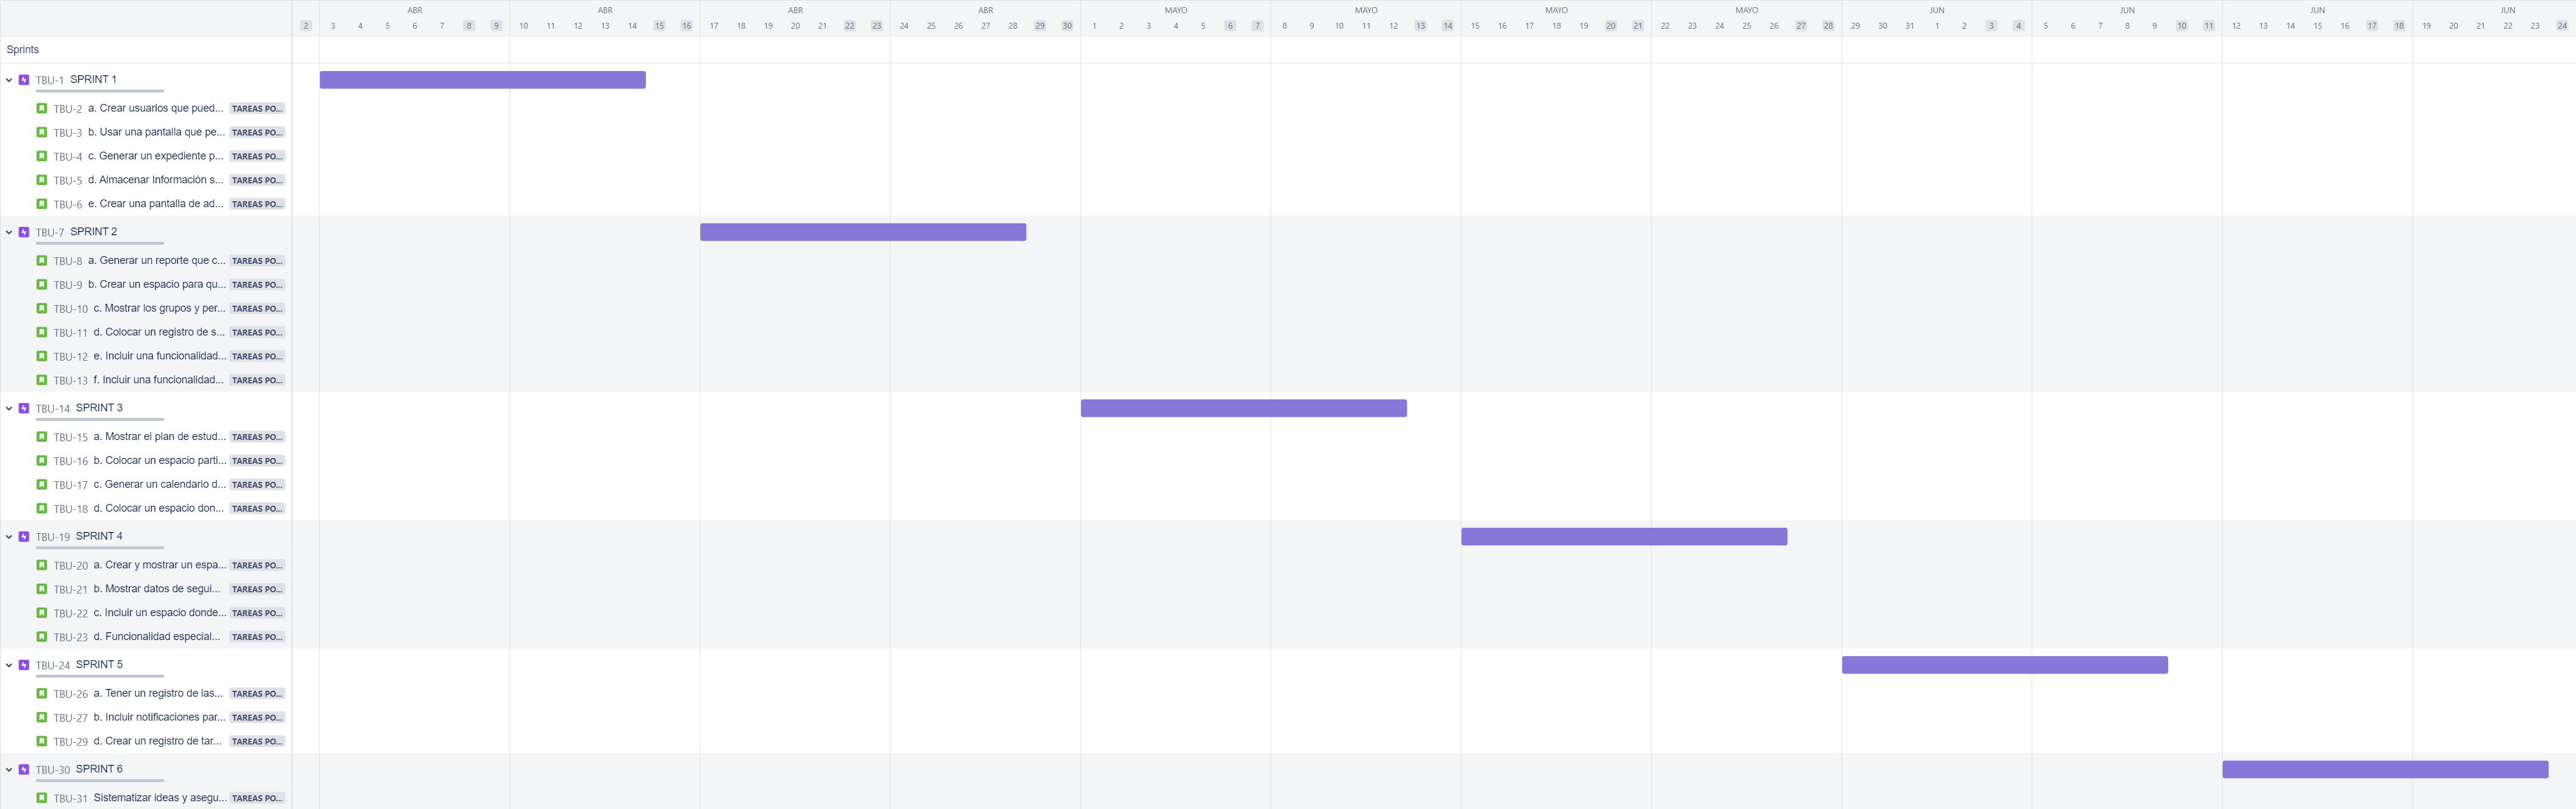
\includegraphics[scale=0.075]{Cronograma_Virtual_Baby.png}
\end{figure}
\end{document}
